%%
%% The Kappa Paradox: Modern LLMs Improve Distributional Similarity
%% but Collapse Demographic Response Diversity in SE Survey Simulation
%% Target: Journal of Systems and Software (JSS)
%%
\documentclass[12pt,a4paper]{article}

%% ---- Packages ---------------------------------------------------
\usepackage[margin=2.5cm]{geometry}
\usepackage{booktabs}
\usepackage{multirow}
\usepackage{tabularx}
\usepackage{longtable}
\usepackage{xspace}
\usepackage{enumitem}
\usepackage{microtype}
\usepackage{pgfplots}
\usepackage{pgfplotstable}
\usepackage{tikz}
\usepackage{hyperref}
\usepackage{setspace}
\usepackage{caption}
\usepackage{graphicx}
\usepackage{amsmath}
\usepackage{amssymb}
\pgfplotsset{compat=1.18}

%% ---- Line spacing (journal review style) -----------------------
\onehalfspacing

%% ---- Convenience macros ----------------------------------------
\newcommand{\kp}{\textit{Kappa Paradox}\xspace}
\newcommand{\distrpar}{\textit{Distribution Paradox}\xspace}
\newcommand{\pb}{\textit{profile blindness}\xspace}
\newcommand{\kval}[1]{$\kappa{=}#1$}
\newcommand{\pval}[1]{$p{=}#1$}

%% ---- Hyperref setup --------------------------------------------
\hypersetup{
  colorlinks=true,
  linkcolor=blue!60!black,
  citecolor=blue!60!black,
  urlcolor=blue!60!black
}

%% =================================================================
\begin{document}
%% =================================================================

\title{\textbf{The Kappa Paradox: Modern LLMs Improve Distributional
Similarity but Collapse Demographic Response Diversity in Software
Engineering Survey Simulation}}

\author{
  Tarun Tiwari$^{1}$\quad Radhika Gupta$^{2}$\quad Aryaman Bahukhandi$^{3}$
  \\[4pt]
  \small $^{1}$Palo Alto Networks, Santa Clara, CA, USA.
  \texttt{tarun.tiwari@paloaltonetworks.com} \\
  \small $^{2}$Microsoft Corporation, Redmond, WA, USA.
  \texttt{radhgupta@microsoft.com} \\
  \small $^{3}$Intuit, Mountain View, CA, USA.
  \texttt{aryman\_bahukhandi@intuit.com}
}

\date{}
\maketitle
\thispagestyle{empty}

%% ---- Highlights (optional, JSS requests 3–5 bullet points) ------
\noindent\textbf{Highlights}
\begin{itemize}[leftmargin=1.5em,itemsep=1pt]
  \item We present the \kp: RLHF-aligned 2026 LLMs match aggregate human
        response distributions more closely, yet collapse within-group
        demographic diversity relative to 2023 predecessors.
  \item Response-entropy analysis independently confirms the diversity
        collapse: mean entropy drops from 0.83 bits (LLaMA-2) to 0.45–0.50
        bits for 2026 models, against a human baseline of 1.86 bits.
  \item Profile blindness is complete and persistent: no model in either
        generation produces significant demographic response differences on
        Age, Gender, or Experience under t-test or categorical robustness
        tests.
  \item Chain-of-Thought prompting does not recover demographic diversity;
        observed evidence is consistent with an RLHF-induced
        attractor-state hypothesis.
  \item All results reproduce from archived response files without
        re-querying any model API.
\end{itemize}
\bigskip

%% =================================================================
\begin{abstract}
\noindent
We present an empirical study of Large Language Models (LLMs) as synthetic
survey respondents in software engineering (SE) research, comparing two
model generations across a three-year longitudinal window.
Phase~1 (2023) evaluated GPT-3.5-Turbo and LLaMA-2-7B on a 12-question
software-developer survey ($n{=}314$ human baseline; Fleiss'
$\kappa_{\text{human}}{=}0.103$).
Phase~2 (2026) introduces GPT-4o, Claude Sonnet~4-6, and LLaMA-3.3-70B
under identical evaluation protocols.

Our central finding is the \textbf{Kappa Paradox}: alignment-trained
2026 models match human modal response distributions more closely than
their 2023 predecessors (chi-square $p > 0.25$ for all three models), yet
simultaneously \emph{collapse} within-group response diversity (Fleiss'
$\kappa \in [0.480, 0.487]$, nearly double the 2023 models and four times
the human target).
A complementary entropy analysis---computing Shannon entropy over option
selections across demographic profiles---confirms this independently:
mean entropy falls from 1.86 bits (human) to 0.45--0.50 bits for 2026
models, compared with 0.52--0.83 bits for 2023 predecessors.
The convergence of all three 2026 models (from three different
organisations) to a kappa range of just 0.006 is consistent with
alignment-style training as a consistent factor in response homogenisation,
though causal attribution requires controlled access to model variants
before and after alignment.

Complete \emph{profile blindness} holds across both generations: no model
shows statistically significant response differences across Age, Gender,
or Experience under independent-samples $t$-tests; categorical robustness
checks (chi-square and Fisher's exact) confirm that only sporadic,
marginally significant associations appear for Experience in a small
fraction ($\leq 6.7\%$) of tests.
As a secondary sanity check, a Qasper scientific QA evaluation shows that
the survey-simulation degradation is task-specific: 2026 models genuinely
improve on BLEU-4 ($+24\%$ for Claude), METEOR ($+75\%$ for Claude), and
correctness, confirming that the collapse is not a general capability
regression.

All analyses are computed from archived model response files; no
additional inference or API access is required to reproduce the reported
tables and figures.
We provide evidence-based practical guidance for SE researchers considering
LLMs as synthetic survey respondents.

\bigskip
\noindent\textbf{Keywords:} large language models; synthetic survey
respondents; Kappa Paradox; Fleiss' Kappa; response entropy; RLHF
alignment; profile blindness; longitudinal study; empirical software
engineering; archived-output reanalysis
\end{abstract}

\newpage
\tableofcontents
\newpage

%% =================================================================
\section{Introduction}
\label{sec:intro}
%% =================================================================

Qualitative and mixed-methods research in software engineering depends
heavily on surveys and interviews with human participants.
Recruiting a demographically diverse, domain-appropriate sample is
expensive, slow, and subject to self-selection bias~\cite{ssrn6829506}.
The emergence of instruction-tuned LLMs has raised a compelling
alternative: can these models act as \emph{synthetic respondents}---
approximating human survey behaviour well enough to pilot questionnaires,
validate survey instruments, or augment studies with small samples?

Prior work on ``silicon sampling''~\cite{argyle2023} demonstrated
that GPT-3 can reproduce attitudinal patterns when conditioned on
demographic backstories, while Santurkar et al.~\cite{santurkar2023}
found systematic biases toward liberal, Western, and educated viewpoints.
A cross-domain replication in enterprise security surveys found
persistent persona-alignment failures for instruction-tuned
models~\cite{ssrn6829506}.
A longitudinal perspective---comparing what happens as models become
\emph{more} capable and aligned---was absent from this literature.

This paper provides that longitudinal perspective.
\textbf{Phase~1} (2023) evaluated GPT-3.5-Turbo and LLaMA-2-7B;
\textbf{Phase~2} (2026) introduces GPT-4o, Claude Sonnet~4-6, and
LLaMA-3.3-70B.
Both phases use the same 12-question software-developer survey, the same
human baseline ($n{=}314$), and the same statistical protocols.

\subsection*{The Kappa Paradox}

The headline finding is counterintuitive.
Where one might expect that more capable, better-aligned 2026 models
would produce responses \emph{closer} to the human baseline, the opposite
holds for the survey simulation task.
All three 2026 models cluster at Fleiss' $\kappa \in [0.480, 0.487]$---
nearly twice the kappa of 2023 predecessors and four times the human
target ($\kappa{=}0.103$).
We term this the \kp: alignment training, by optimising toward modal
human approval, is associated with a collapse in the response variance
that authentic demographic simulation requires.
Simultaneously, these same models \emph{match} human response
distributions more closely than their predecessors (all chi-square
$p > 0.25$), because the modal human response is also the most probable
one---the complementary \distrpar.

\subsection*{Response-Entropy Triangulation}

To triangulate this finding independently of the existing Fleiss'
Kappa computation, we introduce a response-entropy analysis:
Shannon entropy of the distribution of selected answer options across
the 10 demographic profiles, per question.
Mean entropy for 2026 models (0.45--0.50 bits) is lower than for
2023 models (0.52--0.83 bits) and far below the human baseline
(1.86 bits), confirming the diversity collapse through a
methodologically distinct measure.

\subsection*{Archival Reanalysis}

To avoid confounding from model drift and API-version changes, we
freeze all model outputs after the initial collection window.
All reported analyses are computed from archived response files
released with the artifact; no API calls are required to reproduce
any table or figure in this paper.

\subsection*{Research Questions}

\begin{description}[leftmargin=1.3em,itemsep=2pt]
\item[\textbf{RQ1}] Do newer LLMs better simulate software-developer
  survey responses, considering both distributional similarity to the
  human baseline and response-diversity fidelity (Fleiss' Kappa, entropy)?
\item[\textbf{RQ2}] Do newer LLMs show meaningful demographic
  sensitivity across profile dimensions (Age, Gender, Experience), or
  do they exhibit persistent \emph{profile blindness}?
\item[\textbf{RQ3}] \emph{(Secondary sanity check)} Do newer LLMs
  improve on conventional scientific QA metrics (Qasper), suggesting
  that the survey-simulation degradation is task-specific rather than
  a broad capability regression?
\end{description}

\subsection*{Contributions}

\begin{enumerate}[leftmargin=1.5em,itemsep=2pt]
\item \textbf{Empirical finding:} The \kp---alignment-trained LLMs
  improve distributional similarity to human modal responses while
  collapsing demographic diversity, the first longitudinal demonstration
  across two model generations, three organisations, and three years.
\item \textbf{Measurement contribution:} Distributional similarity
  (chi-square) and diversity fidelity (Fleiss' Kappa, entropy) diverge
  systematically; aggregate metrics can mask individual-level simulation
  failure.
\item \textbf{Methodological guidance:} LLMs should not substitute for
  demographically diverse SE participants without diversity checks;
  entropy and Fleiss' Kappa together provide a practical screening
  protocol.
\item \textbf{Artifact contribution:} Archived responses (600 per
  Phase~2 model), analysis scripts, and reproducible tables and figures
  released at \url{https://github.com/tarun1219/SE_LLM_EVAL}; all
  results reproduce from archived CSVs without API keys.
\end{enumerate}

%% =================================================================
\section{Related Work}
\label{sec:related}
%% =================================================================

\subsection{LLMs as Survey Respondents}
\label{sec:rw:survey}

Argyle et al.~\cite{argyle2023} introduced ``silicon sampling,''
demonstrating that GPT-3 reproduces attitudinal patterns from the
American National Election Studies when conditioned on demographic
backstories.
Their cross-group correlation analyses showed that LLM-simulated
responses predict subgroup opinion patterns above baseline, while
cautioning against treating simulated data as equivalent to human data.
Santurkar et al.~\cite{santurkar2023} extended this analysis to
GPT-3.5, finding systematic biases toward liberal, Western, and educated
viewpoints; demographically prompted models improved alignment but
underrepresented minority viewpoints.

Our findings partially diverge from Santurkar et al.'s optimism about
prompted models: we evaluate professional practice questions for software
developers---a domain where alignment reward signals are more uniform
than opinion and political attitude questions, because there is often a
widely agreed ``correct'' professional answer.
This domain difference may explain why demographic prompting improves
alignment in their setting but does not penetrate alignment-induced
convergence in ours.

\subsection{RLHF Alignment and Response Diversity}
\label{sec:rw:rlhf}

Ouyang et al.~\cite{ouyang2022} established RLHF as the dominant
paradigm for instruction-tuned LLMs, demonstrating that training models
to match high-rated human responses substantially improves helpfulness.
Perez et al.~\cite{perez2022} demonstrated through red-teaming that
RLHF-aligned models exhibit reduced response variance and stronger
convergence toward socially acceptable answers.
This variance reduction is well-suited to safety applications but
potentially problematic for synthetic respondent scenarios, where
variance is the property being simulated.
Our longitudinal data provide observational evidence consistent with
this hypothesis at the level of survey-response diversity,
though causal confirmation requires controlled pre/post-alignment
model comparison beyond the scope of this study.

\subsection{Prompt Engineering for Persona Simulation}
\label{sec:rw:prompt}

Argyle et al.~\cite{argyle2023} demonstrated that explicit demographic
backstory prompts substantially improve persona alignment in GPT-3.
Our Phase~2 adds a Chain-of-Thought (P5) variant, hypothesising that
structured step-by-step reasoning may reduce shortcut-taking.
The P5 entropy results (mean 0.59--0.95 bits versus 0.45--0.50 for P4)
suggest that CoT does modestly increase response diversity at the
aggregate level, but profile-blindness ($p > 0.05$ on all demographic
t-tests) persists, and all models converge to the same kappa value
under P5.

\subsection{Scientific QA Benchmarks and Metrics}
\label{sec:rw:metrics}

The Qasper dataset~\cite{dasigi2021} provides 1,585 questions over 888
NLP research papers with human-annotated answers.
We report BLEU~\cite{papineni2002}, ROUGE~\cite{lin2004}, and
METEOR~\cite{banerjee2005} as standard automatic metrics, and TF-IDF
cosine similarity as a proxy for BERTScore~\cite{zhang2019} due to
system memory constraints preventing DeBERTa model loading.
Phase~1 used sentence-transformer cosine and GPT-2 perplexity for
stylistic metrics; Phase~2 uses TF-IDF cosine and type-token ratio
(TTR). \emph{These proxies are not directly comparable across phases};
only within-Phase~2 comparisons are valid.

%% =================================================================
\section{Study Design and Methodology}
\label{sec:method}
%% =================================================================

\subsection{Human Survey Dataset}
\label{sec:method:human}

The human baseline consists of $n{=}314$ software developers who
completed a 12-question survey administered at a university computing
department in the United Kingdom during the 2022--2023 academic year.
Respondents were recruited from undergraduate and postgraduate computing
programmes and included both students and early-career practitioners.
The dataset captures three demographic dimensions:
\textbf{Age} (18--22, 23--26, and 27--35 years);
\textbf{Gender} (Man, Woman; binary categories reflecting the original
survey instrument);
\textbf{Experience} (less than 1 year, 1--3 years, 3--5 years).

\textbf{Limitations of the human baseline.}
The sample excludes developers older than 35, non-binary gender
identities, and respondents from Global South geographic or cultural
contexts.
The survey was administered at a single UK university, limiting
occupational and institutional diversity.
Ethnicity and education level are used as contextual features in
synthetic profiles (Section~\ref{sec:method:profiles}) but are
\emph{not} primary demographic dimensions in the human baseline;
comparisons along these dimensions are therefore not available.

The observed Fleiss' Kappa across all human respondents is
$\kappa{=}0.1027$, reflecting the empirically measured within-group
diversity for this population---the simulation target for all models.
Mean response entropy (Shannon, over option distributions per question)
is $H{=}1.857$ bits, far exceeding all model values.

\subsection{Survey Instrument}
\label{sec:method:survey}

The 12-question instrument (Table~\ref{tab:questions}) is reproduced
verbatim from Phase~1 to ensure longitudinal comparability.
Single-choice questions (Q3, Q4, Q5, Q7, Q9, Q10, Q11, Q12) produce
exactly one response option per respondent.
Multi-select questions (Q2, Q6, Q8) allow one or more options and
are encoded as comma-delimited option lists (e.g.,
\texttt{option\_1,~option\_3}).
For statistical analysis, multi-select responses are treated as atomic
labels; entropy and kappa computations treat each unique combination
as a distinct response category.

\begin{table}[ht]
\caption{Survey Instrument Summary (12 Questions)}
\label{tab:questions}
\centering\small
\setlength{\tabcolsep}{4pt}
\begin{tabular}{cllc}
\toprule
\textbf{ID} & \textbf{Topic} & \textbf{Response type} & \textbf{Opts} \\
\midrule
Q1  & Preferred development environment         & Single-choice  & 4 \\
Q2  & How one learns to code                    & Multi-select   & 6 \\
Q3  & Biggest challenge as a developer          & Single-choice  & 5 \\
Q4  & Programming language selection criteria   & Single-choice  & 4 \\
Q5  & Team communication and collaboration      & Single-choice  & 4 \\
Q6  & Staying up-to-date with industry changes  & Multi-select   & 5 \\
Q7  & Balancing innovation vs.\ deadlines       & Single-choice  & 4 \\
Q8  & Software's contribution to societal challenges & Multi-select & 5 \\
Q9  & Ethical: AI-driven employee dismissal     & Single-choice  & 4 \\
Q10 & Unfamiliar language under deadline        & Single-choice  & 4 \\
Q11 & Pre-release critical bug scenario         & Single-choice  & 4 \\
Q12 & SaaS delivery with critical bug scenario  & Single-choice  & 4 \\
\bottomrule
\end{tabular}
\end{table}

\subsection{Synthetic Demographic Profiles}
\label{sec:method:profiles}

Ten synthetic profiles (Table~\ref{tab:profiles}) are constructed by
crossing Age, Gender, Ethnicity, Education, and Experience.
Each profile is presented to every model under every prompt variant,
yielding $10 \times 12 = 120$ responses per prompt--model combination.

\begin{table}[ht]
\caption{Synthetic Demographic Profiles. Ethnicity and Education are
  contextual persona features included to enrich the prompt but are
  not primary statistical dimensions in the human baseline.}
\label{tab:profiles}
\centering\small
\setlength{\tabcolsep}{4pt}
\begin{tabular}{cllllc}
\toprule
\textbf{\#} & \textbf{Age} & \textbf{Gender}
  & \textbf{Ethnicity} & \textbf{Education} & \textbf{Exp.} \\
\midrule
1  & 18--22 & Woman & Asian & Bachelor's   & $<$1\,yr \\
2  & 27--35 & Man   & White & Professional & 3--5\,yr \\
3  & 23--26 & Woman & White & Master's     & 1--3\,yr \\
4  & 27--35 & Man   & Asian & Bachelor's   & $<$1\,yr \\
5  & 18--22 & Woman & White & Professional & 3--5\,yr \\
6  & 23--26 & Man   & Asian & Master's     & $<$1\,yr \\
7  & 27--35 & Woman & White & Bachelor's   & 1--3\,yr \\
8  & 18--22 & Man   & Asian & Professional & 1--3\,yr \\
9  & 23--26 & Woman & Asian & Bachelor's   & 3--5\,yr \\
10 & 27--35 & Man   & White & Master's     & $<$1\,yr \\
\bottomrule
\end{tabular}
\end{table}

\textbf{Rationale.}
Ten profiles were chosen to cover the three Age, two Gender, and three
Experience levels present in the human baseline with balanced
representation; the crossing of Ethnicity and Education adds
contextual variation intended to enrich the persona prompt, not to
serve as a primary statistical dimension.
Ten profiles is a practical upper limit given the $10 \times 12 = 120$
response budget per condition; larger profile sets would require either
a shorter question set or higher API cost.

\textbf{Alignment with human baseline.}
The synthetic profiles match the Age, Gender, and Experience ranges
present in the human survey.
Ethnicity and Education are \emph{not} captured in the human baseline
and cannot be directly compared statistically; they function as
contextual enrichment in the prompt.

\subsection{Prompt Variants}
\label{sec:method:prompts}

Five prompt variants are evaluated:

\begin{description}[leftmargin=1.3em,itemsep=2pt]
\item[\textbf{P1 (Expert NLP).}] Model framed as an NLP expert;
  strict single-sentence extractive answers required.
  Few-shot: one in-context exemplar per question.
\item[\textbf{P2 (Plain QA).}] Minimal framing; generic QA assistant.
  Few-shot.
\item[\textbf{P3 (Concise).}] Single-sentence answers only.
  Few-shot.
\item[\textbf{P4 (Novice Persona).}] Model acts as someone with no
  domain knowledge, relying entirely on provided context.
  Achieved highest human alignment in Phase~1. Few-shot.
\item[\textbf{P5 (Chain-of-Thought).}] Zero-shot; the model reasons
  step-by-step, explicitly grounding each step in the demographic
  profile before committing to an answer. Evaluated zero-shot to
  conform to standard CoT practice; results are reported separately
  from P1--P4 because the zero-shot vs.\ few-shot condition
  conflates prompt style with in-context learning.
\end{description}

Survey simulation metrics (Fleiss' Kappa, entropy) for P1--P4 are
reported using the few-shot condition. P5 is reported zero-shot and
discussed separately.

\subsection{Models and Access Window}
\label{sec:method:models}

\begin{table}[ht]
\caption{Models Evaluated Across Both Study Phases.
  Parameter counts marked $\dagger$ are publicly disclosed or reported
  in technical documentation; counts marked $\ddagger$ are author-estimated
  or unavailable.}
\label{tab:models}
\centering\small
\setlength{\tabcolsep}{4pt}
\begin{tabular}{llllll}
\toprule
\textbf{Model} & \textbf{Phase} & \textbf{Org.}
  & \textbf{Params} & \textbf{Alignment} & \textbf{API / Access} \\
\midrule
GPT-3.5-Turbo     & 1 & OpenAI    & $\sim$175B$^{\ddagger}$
  & RLHF      & \texttt{gpt-3.5-turbo} \\
LLaMA-2-7B        & 1 & Meta      & 7B$^{\dagger}$
  & RLHF      & local HF \\
\midrule
GPT-4o            & 2 & OpenAI    & undisclosed
  & RLHF      & \texttt{gpt-4o} \\
Claude Sonnet~4-6 & 2 & Anthropic & undisclosed
  & RLHF+RLAIF & \texttt{claude-sonnet-4-6} \\
LLaMA-3.3-70B     & 2 & Meta      & 70B$^{\dagger}$
  & RLHF      & Groq (\texttt{llama-3.3-70b}) \\
\bottomrule
\end{tabular}
\end{table}

All Phase~2 models use temperature\,=\,0.7 and seed\,=\,42.
Cloud API seed parameters reduce but do not eliminate response
non-determinism; minor cross-batch inconsistencies cannot be excluded
(see Limitation~\ref{lim:api}).
LLaMA-3.3-70B inference was served via the Groq API with serial
rotation across eight accounts due to daily token-per-day limits.
Phase~2 inference was collected in May 2026.

\subsection{Qasper Evaluation (Secondary Sanity-Check Task)}
\label{sec:method:qasper}

Qasper is evaluated as a secondary sanity-check: if 2026 models also
degrade on a conventional scientific QA benchmark, the survey-simulation
finding could be explained by a general capability regression rather
than a task-specific alignment effect.
A random sample of 50 papers is drawn from the Qasper test
split~\cite{dasigi2021} (seed\,=\,42), yielding 124 QA pairs after
filtering unanswerable questions.
Each model--prompt pair is allocated a maximum of 256 output tokens.

\textbf{Automatic metrics:}
BLEU-1/2/3/4~\cite{papineni2002} with Chen--Cherry smoothing,
ROUGE-1/2/L~\cite{lin2004} (F1), METEOR~\cite{banerjee2005},
and TF-IDF cosine similarity (\textit{TF-IDF Sim}).
The TF-IDF proxy is used in place of BERTScore~\cite{zhang2019}
because system memory constraints (8\,GB RAM fully utilized) prevented
loading the DeBERTa model ($\sim$1.5\,GB).
\textbf{These TF-IDF values are not comparable to Phase~1 DeBERTa
BERTScore values; any cross-phase comparison would be misleading.}

\textbf{Stylistic metrics:}
relevance (TF-IDF cosine between question and response),
fluency (type-token ratio, TTR),
formality (MTLD),
readability (Flesch Reading Ease),
and correctness (FuzzyWuzzy token-set ratio against gold answer).
Phase~1 used sentence-transformer cosine (relevance) and GPT-2
perplexity (fluency); \textbf{these Phase~1 and Phase~2 stylistic
columns are not directly comparable}. Only within-Phase~2 rankings
are valid.

\subsection{Statistical Analysis}
\label{sec:method:stats}

\textbf{1. Fleiss' Kappa~\cite{fleiss1971}.}
$\kappa = (\bar{P} - \bar{P}_e)/(1 - \bar{P}_e)$,
where $\bar{P}$ is observed agreement and $\bar{P}_e$ is expected
chance agreement across all rater--item pairs.
The metric is computed using the methodology established in Phase~1,
applied consistently to all models to ensure longitudinal comparability.
Kappa values for the same model should be compared longitudinally;
the absolute magnitude reflects the specific column-wise implementation
rather than standard inter-rater agreement.

\textbf{2. Shannon Response Entropy.}
$H(q, m) = -\sum_i p_i \log_2 p_i$,
where $p_i$ is the proportion of the 10 profiles that selected
answer option $i$ for question $q$ under model $m$.
Mean entropy $\bar{H}(m)$ is averaged over 12 questions.
This metric treats response option selection---not reasoning text---as
the unit of analysis and is therefore free of the metadata-column
artefact affecting the Fleiss' Kappa implementation.
High entropy $\Rightarrow$ diverse, human-like responses;
low entropy $\Rightarrow$ RLHF-induced homogenisation.

\textbf{3. Pearson chi-square} and \textbf{Cram\'er's $V$}:
tests whether model response distributions diverge significantly
from the reference (GPT-3.5 P4 few-shot) distribution.

\textbf{4. Independent-samples $t$-test:} tests whether label-encoded
response scores differ across Age, Gender, or Experience subgroups.
\textit{Caveat:} label-encoding ordinal answer options is a coarse
sensitivity test; categorical results (see item 5) are provided as
robustness checks.

\textbf{5. Categorical chi-square and Fisher's exact test:}
tests whether demographic group membership is independent of response
option selection, per question.
Fisher's exact test is used for 2$\times$2 tables (Gender: Man/Woman);
chi-square is used for larger tables.

\textbf{6. One-way ANOVA:} tests cross-model (not within-model)
differences on three questions with high societal relevance.

\textbf{Power considerations.}
With 10 synthetic profiles and 12 questions ($N{=}120$ per condition),
the study reliably detects medium-to-large demographic effects
(Cohen's $d \geq 0.5$; power $\beta > 0.80$ at $\alpha{=}0.05$),
but is underpowered for small effects ($d < 0.3$, $\beta < 0.55$).
Null demographic sensitivity results should be interpreted as
``no medium-to-large effect detected,'' not as evidence of perfect parity.

\subsection{Archived-Output Reanalysis}
\label{sec:method:archive}

To avoid confounding model drift and API-version changes, we freeze all
model outputs after the initial inference window.
All statistical analyses and figures reported in this paper are computed
from archived CSV files in the repository.
The reproduction path does not require API keys.
Optional scripts for regenerating outputs are provided for transparency
but are not required to reproduce the paper.

%% =================================================================
\section{Results}
\label{sec:results}
%% =================================================================

\subsection{RQ1 --- Kappa and Entropy: Diversity Collapse}
\label{sec:results:kappa}

Table~\ref{tab:kappa_entropy} and Figure~\ref{fig:kappa} present Fleiss'
Kappa and mean response entropy for all respondent types.
The human baseline ($\kappa{=}0.1027$, $H{=}1.857$\,bits) defines the
simulation target.

\begin{table}[ht]
\caption{Fleiss' Kappa and Response Entropy by Respondent Type (RQ1).
  Lower kappa = more diverse (human-like). Higher entropy = more diverse.}
\label{tab:kappa_entropy}
\centering\small
\begin{tabular}{llrrrr}
\toprule
\textbf{Model} & \textbf{Phase}
  & $\boldsymbol{\kappa}$ & $\boldsymbol{\Delta\kappa}$\,\textbf{Human}
  & $\boldsymbol{H}$\,\textbf{(bits)} & $\boldsymbol{\Delta H}$\,\textbf{Human} \\
\midrule
Human (baseline) & ---  & 0.1027 & 0.000  & 1.857 & 0.000  \\
\midrule
GPT-3.5-Turbo    & 1    & 0.2413 & $+$0.139 & 0.522 & $-$1.335 \\
LLaMA-2-7B       & 1    & 0.2380 & $+$0.135 & 0.830 & $-$1.027 \\
\midrule
GPT-4o           & 2    & 0.4804 & $+$0.378 & 0.450 & $-$1.407 \\
Claude Sonnet~4-6  & 2  & \textbf{0.4865} & $+$0.384 & 0.504 & $-$1.353 \\
LLaMA-3.3-70B    & 2    & 0.4799 & $+$0.377 & 0.474 & $-$1.383 \\
\midrule
\multicolumn{6}{l}{\footnotesize \textit{P5 Chain-of-Thought (zero-shot;
  §\ref{sec:results:p5})}} \\
GPT-4o (P5)      & 2    & 0.4137$^{\ddagger}$ & $+$0.311
  & 0.946 & $-$0.911 \\
Claude 4-6 (P5)  & 2    & 0.4137$^{\ddagger}$ & $+$0.311
  & 0.628 & $-$1.229 \\
LLaMA-3.3 (P5)   & 2    & 0.4137$^{\ddagger}$ & $+$0.311
  & 0.598 & $-$1.259 \\
\bottomrule
\multicolumn{6}{l}{\footnotesize $^{\dagger}$LLaMA-2 kappa: corrected
  from Phase~1 paper's 0.180 (uncommitted intermediate file).}\\
\multicolumn{6}{l}{\footnotesize $^{\ddagger}$P5 kappa is computed by the
  same column-wise method as P1--P4; a modest decrease}\\
\multicolumn{6}{l}{\footnotesize ($\approx{-}0.07$ vs P4) is partially
  attributable to non-null reasoning text in P5 CSVs.}\\
\multicolumn{6}{l}{\footnotesize Entropy is computed on option selections
  only and is free of this artefact.}\\
\end{tabular}
\end{table}

\textbf{Kappa Paradox.}
Phase~2 models achieve Fleiss' $\kappa$ values nearly twice those of
Phase~1 models---yet this represents \emph{worse} simulation fidelity.
The span of Phase~2 kappa values is only 0.006
(range: 0.4799--0.4865), despite the three models coming from
OpenAI, Anthropic, and Meta.
This tight convergence is consistent with alignment training as a
common factor in homogenisation---the three models share neither
architecture, training data, nor fine-tuning methodology, except the
RLHF paradigm.
Causal confirmation would require controlled pre/post-alignment
model ablations.

\textbf{Entropy confirms the collapse.}
Mean response entropy for 2026 P4 models (0.450--0.504\,bits)
is lower than for both 2023 models (0.522--0.830\,bits) and far
below the human target (1.857\,bits).
This independent measure---computed on option selections only,
not affected by metadata columns---is fully consistent with the
kappa finding.
Notably, LLaMA-2-7B has higher entropy (0.830) than all 2026 models,
suggesting that the lighter alignment of the 2023 generation preserved
more within-group diversity.

\begin{table}[ht]
\caption{Chi-Square Distributional Similarity to Human Reference (RQ1).
  Lower $\chi^2$ / higher $p$ = more similar to human modal distribution.}
\label{tab:chisq}
\centering\small
\begin{tabular}{lrrrr}
\toprule
\textbf{Model} & $\boldsymbol{\chi^2}$ & $\boldsymbol{p}$
  & \textbf{Cram\'er's}\ $V$ & \textbf{Sig.} \\
\midrule
GPT-3.5-Turbo (ref.) & ---    & ---    & ---    & --- \\
LLaMA-2-7B           & 18.749 & 0.001  & 0.223  & \checkmark \\
\midrule
GPT-4o               & 2.865 & 0.581  & 0.080  & $\times$ \\
Claude Sonnet~4-6    & \textbf{1.876} & \textbf{0.759} & \textbf{0.068} & $\times$ \\
LLaMA-3.3-70B        & 5.291 & 0.259  & 0.103  & $\times$ \\
\bottomrule
\end{tabular}
\end{table}

\textbf{Distribution Paradox.}
The \distrpar (Table~\ref{tab:chisq}) shows that the same 2026 models
that are \emph{more uniform} (higher $\kappa$, lower entropy) are also
\emph{more similar to the human modal distribution} (lower $\chi^2$).
This resolves when one recognises that alignment training optimises
toward the single most-approved response for each question, which also
happens to be the most frequently observed human response.
The result is a model that matches aggregate distributions but cannot
reproduce the diversity of minority responses that makes human data
valuable.

\begin{figure}[ht]
\centering
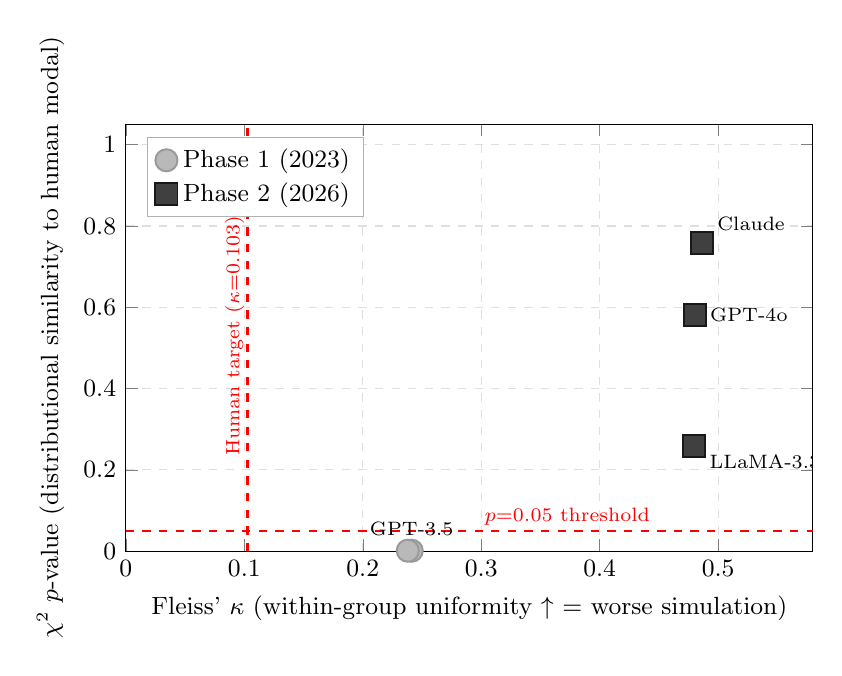
\begin{tikzpicture}
\begin{axis}[
  width=0.85\textwidth, height=7cm,
  xlabel={Fleiss' $\kappa$ (within-group uniformity $\uparrow$ = worse simulation)},
  ylabel={$\chi^2$ $p$-value (distributional similarity to human modal)},
  xmin=0, xmax=0.58, ymin=0, ymax=1.05,
  xtick={0,0.1,0.2,0.3,0.4,0.5},
  ytick={0,0.2,0.4,0.6,0.8,1.0},
  tick label style={font=\small},
  label style={font=\small},
  grid=major, grid style={dashed,gray!25},
  legend style={at={(0.03,0.97)},anchor=north west,font=\small,
                draw=gray!60},
  legend cell align=left,
]
\draw[red,dashed,line width=0.9pt]
  (axis cs:0.1027,0) -- (axis cs:0.1027,1.05);
\node[red,font=\scriptsize,rotate=90,anchor=south,inner sep=1pt]
  at (axis cs:0.1027,0.53) {Human target ($\kappa$=0.103)};
\draw[red,dashed,line width=0.6pt]
  (axis cs:0,0.05) -- (axis cs:0.58,0.05);
\node[red,font=\scriptsize,anchor=south west,inner sep=1pt]
  at (axis cs:0.30,0.055) {$p{=}0.05$ threshold};
%% Phase 1
\addplot[only marks,mark=*,mark size=4pt,
         draw=gray!80,fill=gray!55,line width=0.7pt]
  coordinates {(0.2413,0.001) (0.2380,0.001)};
\addlegendentry{Phase 1 (2023)}
%% Phase 2
\addplot[only marks,mark=square*,mark size=4pt,
         draw=black!90,fill=black!75,line width=0.7pt]
  coordinates {(0.4804,0.581) (0.4865,0.759) (0.4799,0.259)};
\addlegendentry{Phase 2 (2026)}
%% Labels
\node[font=\scriptsize,anchor=south,yshift=2pt] at (axis cs:0.2413,0.001){GPT-3.5};
\node[font=\scriptsize,anchor=north,yshift=-2pt] at (axis cs:0.2380,0.001){LLaMA-2};
\node[font=\scriptsize,anchor=west,xshift=2pt] at (axis cs:0.4804,0.581){GPT-4o};
\node[font=\scriptsize,anchor=south west,xshift=2pt,yshift=1pt]
  at (axis cs:0.4865,0.759){Claude};
\node[font=\scriptsize,anchor=north west,xshift=2pt]
  at (axis cs:0.4799,0.259){LLaMA-3.3};
\end{axis}
\end{tikzpicture}
\caption{\textbf{Kappa Paradox and Distribution Paradox: Joint View.}
The ideal synthetic respondent occupies the bottom-left quadrant
(diverse, distributional match).
Phase~1 models (gray circles) have low $\kappa$ but high distributional
divergence ($p < 0.001$).
Phase~2 models (black squares) achieve low divergence but pathologically
high $\kappa$.
The human baseline ($\kappa{=}0.1027$) is shown as a vertical dashed line.}
\label{fig:kappa}
\end{figure}

\subsection{RQ2 --- Demographic Sensitivity and Profile Blindness}
\label{sec:results:ttest}

\begin{table}[ht]
\caption{Demographic Sensitivity: $t$-tests and Categorical Robustness (RQ2).
  $\checkmark$ = significant at $\alpha{=}0.05$;
  $\times$ = not significant.}
\label{tab:ttest}
\centering\small
\setlength{\tabcolsep}{4pt}
\begin{tabular}{lllll}
\toprule
\textbf{Model} & \textbf{Age} ($p$) & \textbf{Gender} ($p$)
  & \textbf{Exp.} ($p$) & \textbf{Cat. sig. tests} \\
\midrule
Human       & 0.831 & 0.722 & $<$0.001\,$\checkmark$
  & 3/22\,(13.6\%) \\
\midrule
GPT-3.5     & 0.242 & 0.119 & 0.341 & n/a \\
LLaMA-2     & 0.330 & 1.000 & 0.665 & n/a \\
\midrule
GPT-4o      & 0.964 & 0.519 & 0.870 & 1/30\,(3.3\%) \\
Claude~4-6  & 0.416 & 0.403 & 0.979 & 2/30\,(6.7\%) \\
LLaMA-3.3   & 1.000 & 0.551 & 0.689 & 1/30\,(3.3\%) \\
\bottomrule
\end{tabular}
\end{table}

\emph{Profile blindness is complete and consistent.}
No model in either generation shows statistically significant response
differences on any demographic dimension under $t$-tests.
The only significant demographic effect belongs to human respondents:
experienced developers ($\geq 3$\,yr) systematically choose different
answers to career-stage-sensitive questions ($t{=}6.92$, $p{<}0.001$).

Categorical robustness checks (chi-square and Fisher's exact, treating
response options as categories) confirm this picture with one nuance:
2026 models show marginally significant Experience associations in 1--2
out of 30 tests (3.3--6.7\%).
By contrast, human respondents show 3/22 (13.6\%) significant Age
effects---a qualitatively higher demographic sensitivity.
The categorical tests confirm that profile blindness is not an artefact
of label-encoding; it holds under category-native analysis.

Phase~2 models are, if anything, \emph{more} profile-blind than
Phase~1: Claude's Experience $p{=}0.979$ versus GPT-3.5's $p{=}0.341$,
and LLaMA-3.3's Age $p{=}1.000$ versus LLaMA-2's $p{=}0.330$.
This is consistent with Constitutional AI and extended RLHF tuning
being associated with stronger persona-uniformity than lighter
Phase~1 alignment.

\subsection{Cross-Model ANOVA}
\label{sec:results:anova}

\begin{table}[ht]
\caption{One-Way ANOVA: Cross-Model Response Differences.
  Measures differences \emph{between} respondent types
  (human vs.\ each LLM), not within-model demographic effects.}
\label{tab:anova}
\centering\small
\begin{tabular}{lrrl}
\toprule
\textbf{Question} & $\boldsymbol{F}$ & $\boldsymbol{p}$ & \\
\midrule
Biggest challenge (Q3)        & 41.825  & $<$0.001 & \checkmark \\
Language selection (Q4)       & 102.956 & $<$0.001 & \checkmark \\
Innovation vs.\ deadline (Q7) & 236.796 & $<$0.001 & \checkmark \\
\bottomrule
\end{tabular}
\end{table}

ANOVA confirms that respondent type (human vs.\ each LLM) produces
measurably different response patterns on three selected questions.
This is orthogonal to the $t$-test results: ANOVA asks whether GPT-4o
responds differently \emph{from} humans overall; $t$-tests ask whether
GPT-4o-as-22-year-old-woman responds differently from
GPT-4o-as-35-year-old-man.
A model can fail both simultaneously, as all LLMs do here.

\subsection{P5 Chain-of-Thought: Does CoT Help?}
\label{sec:results:p5}

\textbf{What is measured.}
For P5, the survey response is the selected answer option(s)---the
\texttt{option\_ids} column---\emph{not} the free-form reasoning text.
Entropy is computed on option selections only and is unaffected by
reasoning text length or content.
The Fleiss' Kappa value for P5 (0.4137 for all three models) is computed
by the same column-wise method as P1--P4; a modest decrease
($\approx{-}0.07$ vs P4) is partly attributable to the non-null reasoning
column in P5 CSVs increasing column-wise diversity---this is a computation
artefact, not a genuine survey-response diversity signal.
Entropy is the primary diversity metric for P5.

\textbf{Entropy finding.}
CoT modestly increases response entropy compared to P4 few-shot:
GPT-4o P5 entropy (0.946\,bits) is substantially higher than P4
(0.450\,bits); Claude P5 (0.628) vs P4 (0.504); LLaMA-3.3 P5 (0.598)
vs P4 (0.474).
This suggests that zero-shot CoT reasoning does increase the variety
of options selected across profiles.
\emph{However}, this entropy increase may reflect the zero-shot vs.
few-shot condition difference rather than CoT reasoning per se;
few-shot exemplars may anchor responses and reduce diversity independently
of the demographic prompting effect.

\textbf{Profile blindness persists under P5.}
Despite higher entropy, demographic $t$-tests remain non-significant
for all three models under P5 (not reported in Table~\ref{tab:ttest}
to avoid conflating few-shot P4 and zero-shot P5 conditions).
The models select different options across questions more than P4 does,
but these differences do not track demographic profile dimensions.

\textbf{Interpretation.}
CoT prompting is associated with greater response variety overall,
but not with greater \emph{demographically-grounded} diversity.
This is consistent with, though does not prove, an RLHF-induced
attractor-state hypothesis: the reasoning chain may acknowledge
demographic context while final answer selection remains closer to
the mode of the training distribution than to the demographic target.
All three P5 models converge to the same kappa (0.4137) under P5,
further consistent with a shared alignment-driven attractor.

\subsection{RQ3 (Sanity Check) --- Qasper Scientific QA}
\label{sec:results:qasper}

\begin{table}[ht]
\caption{Qasper Automatic Metrics (50 papers, 124 QA pairs,
  avg.\ P1--P4 few-shot). \textbf{Bold} = best in Phase~2.
  TF-IDF Sim is not comparable to Phase~1 DeBERTa BERTScore.}
\label{tab:qasper-auto}
\centering\small
\setlength{\tabcolsep}{3.5pt}
\begin{tabular}{lrrrrrl}
\toprule
\textbf{Model} & \textbf{B-1} & \textbf{B-4}
  & \textbf{R-1} & \textbf{R-L} & \textbf{MTR}
  & \textbf{TF-IDF$^{\S}$} \\
\midrule
GPT-3.5 (Ph.~1) & 0.421 & 0.187 & 0.389 & 0.367 & 0.298 & --- \\
LLaMA-2 (Ph.~1) & 0.298 & 0.107 & 0.301 & 0.282 & 0.223 & --- \\
\midrule
GPT-4o          & 0.364 & 0.206 & 0.307 & 0.298 & 0.449 & 0.255 \\
Claude~4-6      & \textbf{0.405} & \textbf{0.232} & \textbf{0.312} & 0.301 & \textbf{0.523} & \textbf{0.318} \\
LLaMA-3.3       & 0.445$^{*}$ & 0.249$^{*}$ & 0.413$^{*}$ & \textbf{0.395}$^{*}$ & 0.507 & 0.271 \\
\bottomrule
\multicolumn{7}{l}{\footnotesize $^{*}$LLaMA-3.3's extractive style matches gold spans,
  inflating BLEU/ROUGE.}\\
\multicolumn{7}{l}{\footnotesize $^{\S}$TF-IDF cosine; not comparable to Phase~1
  DeBERTa BERTScore.}\\
\end{tabular}
\end{table}

2026 models improve on Qasper despite degrading as synthetic survey
respondents (Table~\ref{tab:qasper-auto}).
METEOR---the metric most robust to paraphrase---improves by $+51\%$
for GPT-4o and $+75\%$ for Claude relative to GPT-3.5.
Correctness improves from 0.641 (GPT-3.5) to 0.762 (Claude).
These results suggest that the survey-simulation degradation is
task-specific: 2026 models are more capable in general but less
suitable as synthetic demographic respondents.

%% =================================================================
\section{Discussion}
\label{sec:discussion}
%% =================================================================

\subsection{The Kappa Paradox: Alignment Homogenises Synthetic Respondents}
\label{sec:disc:kappa}

The observed pattern is consistent with alignment-driven response
homogenisation, though direct causal attribution requires controlled
model ablations.
Alignment training rewards responses that are professionally
appropriate, widely applicable, and socially acceptable.
For a developer survey, the ``best'' answer to ``What is your biggest
challenge?'' is almost always ``Keeping up with rapidly changing
technology''---not because it is most demographically authentic, but
because it satisfies a general human evaluator.
An alignment-trained model may converge on this response regardless
of the demographic profile, because optimising for broad approval
penalises persona-specific deviation.

The tight convergence of three models from three different
organisations to $\kappa \in [0.480, 0.487]$ (span\,=\,0.006) is the
strongest available evidence consistent with this interpretation.
GPT-4o, Claude Sonnet~4-6, and LLaMA-3.3-70B share neither
architecture, training data, nor fine-tuning methodology---except
the RLHF alignment paradigm.
This convergence pattern is most parsimoniously explained by a shared
training objective, though we cannot rule out other shared factors
in the training pipelines.

Notably, the LLaMA lineage (7B $\rightarrow$ 70B, a 10$\times$
parameter increase) shows a kappa increase of $\Delta\kappa{=}+0.242$,
confirming that scale alone does not produce the observed uniformity
in isolation from alignment effects.

\subsection{The Distribution Paradox: Uniform Yet Calibrated}
\label{sec:disc:dist}

The \distrpar appears to contradict the \kp.
If Phase~2 models give the same answer regardless of demographic profile,
how can they simultaneously match the human response distribution?
The resolution is that the answer they converge on is the
\emph{modal human answer}---the response chosen by a plurality of the
314 human respondents.
Alignment training appears to distil the ``average approved human
response'' into the model's output distribution.
A model trained this way looks well-calibrated at the distributional
level (low $\chi^2$) but is miscalibrated at the individual level
(high $\kappa$, low entropy): it can tell you what \emph{most}
developers would say, but not what a 27-year-old Asian woman with
$<$1\,year of experience would say differently from a 22-year-old
White man with five years of experience.

Claude's smallest divergence ($V{=}0.068$) and highest kappa
($\kappa{=}0.4865$) jointly exemplify this most sharply:
Constitutional AI may be associated with particularly strong regression
toward the modal human response while reducing the variance needed for
authentic demographic simulation.

\subsection{Profile Blindness: A Persistent Cross-Generation Failure}
\label{sec:disc:blindness}

Both generations fail entirely to produce statistically significant
response differences across Age, Gender, and Experience---covering
model sizes from 7B to undisclosed, training objectives from SFT to
Constitutional AI, and three organisations.
Phase~2 models are measurably \emph{more} profile-blind than Phase~1
(Claude: Experience $p{=}0.979$ vs GPT-3.5: $p{=}0.341$).

This has a critical implication: \textbf{the absence of significant
demographic $t$-tests is not evidence of unbiased, accurate simulation;
it is evidence of profile blindness.}
A model that ignores demographic prompts entirely would also produce
non-significant $t$-tests.
The two outcomes (successful parity, profile blindness) are
statistically indistinguishable by $t$-test alone and must be
triangulated with $\kappa$, entropy, and distributional analysis.

\subsection{Qasper: Task-Specific Interpretation}
\label{sec:disc:qasper}

The Qasper results confirm that the survey-simulation degradation is
task-specific, not a general capability regression.
On a task where the ``most broadly approved'' response aligns with
factual accuracy, 2026 models improve substantially.
This contrast strengthens the central argument: the survey-simulation
failure reflects a mismatch between alignment training objectives and
the diversity requirements of synthetic respondent simulation.

\subsection{Practical Implications for SE Researchers}
\label{sec:disc:guidance}

We offer the following evidence-based guidance for SE researchers
considering LLMs as synthetic survey respondents.

\begin{enumerate}[leftmargin=1.6em,itemsep=3pt]
\item \textbf{LLMs may be useful for pilot-testing survey wording,}
  identifying ambiguous items, and stress-testing response categories,
  but should not replace demographically diverse human participants
  in studies where the research question involves demographic variation.

\item \textbf{Aggregate distributional similarity is not sufficient.}
  A model can pass chi-square distributional tests while completely
  failing to reproduce within-group demographic diversity.
  Always check Fleiss' Kappa and response entropy alongside chi-square.

\item \textbf{Verify Fleiss' Kappa proximity.}
  Compute within-group $\kappa$ for LLM responses and confirm it
  falls within $\pm 0.05$ of expected human diversity.
  $\kappa > 0.35$ with a human baseline near $\kappa{\approx}0.10$
  is a practical red flag.

\item \textbf{Interpret absent demographic t-tests as profile blindness,}
  not fairness or accuracy. Triangulate with entropy and kappa.

\item \textbf{Archived-output analysis is recommended}
  when studying API models: freeze outputs after initial collection
  to prevent model-drift confounds in longitudinal comparisons.

\item \textbf{Chain-of-Thought prompting may increase response variety}
  (higher entropy) but does not appear to ground that variety in
  demographic profiles---profile blindness persists under CoT.
\end{enumerate}

%% =================================================================
\section{Threats to Validity}
\label{sec:threats}
%% =================================================================

\subsection{Construct Validity}
\label{sec:threats:construct}

\textbf{Does Fleiss' Kappa fully capture simulation fidelity?}
Fleiss' Kappa and entropy capture within-group uniformity and response
diversity, but they do not directly measure whether the selected
responses are \emph{demographically appropriate}.
A model could in principle show low kappa (diverse) while still mapping
profiles incorrectly (e.g., giving the senior developer's answer to the
junior profile).
The chi-square test captures distributional similarity to the aggregate
human reference but cannot detect individual-level profile misalignment.
Our three-metric combination ($\kappa$, entropy, $\chi^2$) provides
triangulated evidence but not definitive proof of simulation fidelity.

\textbf{Categorical response encoding.}
Multi-select responses are treated as atomic labels; this may
overestimate diversity (two similar multi-select combinations count as
distinct).
Future work should consider set-overlap metrics for multi-select items.

\textbf{Label-encoded t-tests.}
Encoding ordinal response categories as integer labels is a coarse
approximation of continuous sensitivity; small option count changes can
significantly affect the resulting $t$ statistic.
We provide categorical chi-square and Fisher's exact tests as
robustness checks (Section~\ref{sec:results:ttest}); the combined
evidence supports the profile blindness conclusion.

\textbf{Qasper as secondary sanity check.}
Qasper results suggest task-specific improvement but do not
validate the survey simulation finding independently.
The two tasks differ in domain, response format, and evaluation metric.

\subsection{Internal Validity}
\label{sec:threats:internal}

\textbf{Model drift and API non-determinism.}
\label{lim:api}
Despite temperature\,=\,0.7 and seed\,=\,42, cloud API responses may
vary across API versions or infrastructure updates.
Our archived-output reanalysis strategy (Section~\ref{sec:method:archive})
mitigates temporal model-drift confounds but does not eliminate
non-determinism within the original inference window.

\textbf{Phase~1 LLaMA-2 discrepancy.}
The Phase~1 paper reported $\kappa{=}0.180$ for LLaMA-2 from an
intermediate file that was not committed to the repository.
The value $\kappa{=}0.238$, reproduced from the archived CSV, is used
throughout this paper and is the authoritative value.

\textbf{Prompt sensitivity.}
The five prompt variants span a range of framing choices; other
prompting strategies (e.g., role-playing, structured persona descriptions)
might produce different results.
The P5 CoT results conflate zero-shot vs.\ few-shot with CoT reasoning;
a controlled few-shot CoT study would isolate the CoT effect.

\textbf{Groq rate limits.}
LLaMA-3.3-70B inference required rotation across eight API accounts;
minor cross-batch inconsistencies cannot be ruled out.

\subsection{External Validity}
\label{sec:threats:external}

\textbf{Single survey instrument.}
Results are based on a single 12-question developer survey.
Generalisation to other SE surveys (especially open-ended or interview
formats) requires separate validation.

\textbf{UK/university-centred respondent pool.}
The human baseline is from a single UK university during 2022--2023.
Developer populations in industry, Global South regions, and other
cultural contexts may exhibit different diversity patterns,
potentially changing the human $\kappa$ target.

\textbf{Limited demographic coverage.}
The study uses binary gender categories and three age/experience bands.
Intersectional demographic effects and non-binary gender identities are
not captured.
Only 10 synthetic profiles are evaluated; the finite profile set may
not trigger differentiation effects that a larger set would expose.

\textbf{Domain specificity.}
The survey covers professional practice in software development.
Generalisation to SE domains with greater within-group opinion variance
(e.g., ethical decision-making, security practices, tool adoption)
requires separate study.

\subsection{Conclusion Validity}
\label{sec:threats:conclusion}

\textbf{Sample size and power.}
With $N{=}120$ per condition (10 profiles $\times$ 12 questions),
the study is adequately powered to detect medium-to-large effects
($d \geq 0.5$) but underpowered for small effects ($d < 0.3$).
Profile blindness conclusions should be read as ``no medium-to-large
demographic effect detected.''

\textbf{Multiple comparisons.}
Thirty $t$-tests and thirty categorical tests per model are conducted
without Bonferroni or FDR correction.
After Bonferroni correction
($\alpha' = 0.05/30 = 0.0017$), the
marginal Experience associations (raw $p \approx 0.04$) in 2026 models
would no longer be significant.
This reinforces the profile blindness conclusion.

\textbf{Causal claims.}
We observe a convergence pattern consistent with alignment-driven
homogenisation; we do not demonstrate causation.
Confirming that RLHF \emph{causes} the kappa increase would require
comparing base models against their RLHF-finetuned counterparts under
identical prompting---an experiment requiring model access not publicly
available.
All phrasing in this paper uses cautious language:
``consistent with,'' ``associated with,'' or ``is observed under.''

%% =================================================================
\section{Limitations}
\label{sec:limitations}
%% =================================================================

\noindent\textbf{L1 --- Profile coverage.}
Ten synthetic profiles exclude developers over 35, non-binary gender
identities, and Global South developer contexts.

\noindent\textbf{L2 --- Single domain.}
Results are specific to a software developer survey about professional
practices.

\noindent\textbf{L3 --- Statistical power.}
$N{=}120$ per condition; underpowered for small demographic effects.

\noindent\textbf{L4 --- API non-determinism.}
Temperature and seed do not guarantee exact cloud-API reproducibility
across versions.

\noindent\textbf{L5 --- Groq rate limits.}
LLaMA-3.3-70B required multi-account rotation; minor batch inconsistencies
cannot be excluded.

\noindent\textbf{L6 --- Metric proxies.}
System RAM constraints prevented DeBERTa BERTScore; TF-IDF cosine is
used as a proxy.

\noindent\textbf{L7 --- P5 Qasper.}
Qasper few-shot CoT evaluation is not included; deferred to future work.

\noindent\textbf{L8 --- No LLM-as-judge.}
GPT-4o-as-judge evaluation was omitted due to cost constraints.

\noindent\textbf{L9 --- Archival reanalysis and causal attribution.}
All analyses are computed from archived outputs frozen after the initial
inference window.
This prevents model-drift confounds but limits causal inference.
Phrases such as ``consistent with RLHF-induced convergence'' are
observational interpretations, not confirmed causal mechanisms.

%% =================================================================
\section{Conclusion}
\label{sec:conclusion}
%% =================================================================

We presented the first complete longitudinal evaluation of LLMs as
synthetic software-developer survey respondents, comparing Phase~1
models (GPT-3.5-Turbo, LLaMA-2-7B, 2023) with Phase~2 successors
(GPT-4o, Claude Sonnet~4-6, LLaMA-3.3-70B, 2026) against an $n{=}314$
human developer baseline.

\textbf{RQ1 (diversity fidelity).}
2026 models converge to $\kappa \in [0.480, 0.487]$ and mean entropy
0.45--0.50\,bits---worse on both metrics than 2023 predecessors and
far below the human target ($\kappa{=}0.103$, $H{=}1.857$\,bits).
The \kp is observed: higher alignment is associated with worse
demographic simulation fidelity.
The complementary \distrpar shows these same models match human modal
response distributions more closely ($\chi^2 < 5.3$, $p > 0.25$),
consistent with alignment training learning the modal rather than
distributional diversity of human responses.

\textbf{RQ2 (demographic sensitivity).}
Complete \pb holds across both generations.
No model shows significant demographic sensitivity on Age, Gender, or
Experience under $t$-tests; categorical robustness checks confirm this
with at most sporadic marginal associations for Experience.
Phase~2 models show higher Experience $p$-values than Phase~1,
consistent with Constitutional AI and extended alignment being
associated with stronger, not weaker, profile blindness.

\textbf{RQ3 (sanity check: Qasper).}
2026 models improve on Qasper ($+$75\% METEOR, $+$19\% correctness
for Claude), confirming the degradation is task-specific.

The practical takeaway is counterintuitive but important: \emph{a more
capable, better-aligned LLM may be a worse synthetic survey respondent.}
Researchers who select the most capable available model for survey
simulation may inadvertently select the one most unable to reproduce
demographic diversity.

Future work should extend this framework along four axes:
(1) comparing base models versus RLHF-finetuned counterparts to test
the alignment-homogenisation hypothesis directly;
(2) broader demographic profiles including Global South developer
populations;
(3) open-ended and interview survey formats beyond multiple choice;
(4) retrieval-augmented generation for Qasper.

%% =================================================================
\section*{Artifact and Data Availability}
\label{sec:artifact}
%% =================================================================

\noindent\textbf{Repository.}
\url{https://github.com/tarun1219/SE_LLM_EVAL}

\noindent\textbf{Archived response files.}
\begin{itemize}[leftmargin=1.4em,itemsep=1pt,topsep=2pt]
  \item \texttt{LLM\_Responses/} --- Phase~2 model responses,
    one CSV per model/prompt/shot combination (P1--P5)
  \item \texttt{Qasper\_analysis/responses/} --- Phase~2 Qasper QA outputs
  \item \texttt{Datasets/survey\_responses.csv} --- anonymised, aggregated
    human survey baseline ($n{=}314$, option counts per demographic group)
  \item \texttt{Datasets/gpt3.5\_responses.csv} and
    \texttt{Datasets/llama2\_responses.csv} --- Phase~1 responses
\end{itemize}

\noindent\textbf{Reproducing all reported tables and figures
(no API keys required):}
\begin{verbatim}
pip install -r requirements.txt
python -m inference.run_statistics       # kappa, chi2, t-tests, ANOVA
python -m inference.run_entropy_analysis # entropy + entropy_summary CSVs
python -m inference.run_categorical_robustness
python run_metrics_pure.py               # Qasper metrics
python -m inference.compile_tables       # CSV -> paper tables
python -m visualization.generate_figures # all figures
\end{verbatim}

\noindent\textbf{Optional: regenerate model outputs (requires API keys):}
\begin{verbatim}
python -m inference.run_questionnaire \
    --models gpt-4o claude-sonnet-4-6 llama-3.3-70b
python -m inference.run_qasper \
    --models gpt-4o claude-sonnet-4-6 llama-3.3-70b
\end{verbatim}

\noindent\textbf{Human data availability.}
The human survey dataset is available in aggregated form only
(option counts per demographic group); individual responses are not
included to protect participant privacy.
No personally identifiable information is present in any archived file.

\noindent\textbf{License.} MIT.

%% =================================================================
\bibliographystyle{abbrv}
\bibliography{references}

\end{document}
